% Options for packages loaded elsewhere
\PassOptionsToPackage{unicode}{hyperref}
\PassOptionsToPackage{hyphens}{url}
%
\documentclass[
  english,
  man,11pt,floatsintext]{apa7}
\usepackage{lmodern}
\usepackage{amssymb,amsmath}
\usepackage{ifxetex,ifluatex}
\ifnum 0\ifxetex 1\fi\ifluatex 1\fi=0 % if pdftex
  \usepackage[T1]{fontenc}
  \usepackage[utf8]{inputenc}
  \usepackage{textcomp} % provide euro and other symbols
\else % if luatex or xetex
  \usepackage{unicode-math}
  \defaultfontfeatures{Scale=MatchLowercase}
  \defaultfontfeatures[\rmfamily]{Ligatures=TeX,Scale=1}
\fi
% Use upquote if available, for straight quotes in verbatim environments
\IfFileExists{upquote.sty}{\usepackage{upquote}}{}
\IfFileExists{microtype.sty}{% use microtype if available
  \usepackage[]{microtype}
  \UseMicrotypeSet[protrusion]{basicmath} % disable protrusion for tt fonts
}{}
\makeatletter
\@ifundefined{KOMAClassName}{% if non-KOMA class
  \IfFileExists{parskip.sty}{%
    \usepackage{parskip}
  }{% else
    \setlength{\parindent}{0pt}
    \setlength{\parskip}{6pt plus 2pt minus 1pt}}
}{% if KOMA class
  \KOMAoptions{parskip=half}}
\makeatother
\usepackage{xcolor}
\IfFileExists{xurl.sty}{\usepackage{xurl}}{} % add URL line breaks if available
\IfFileExists{bookmark.sty}{\usepackage{bookmark}}{\usepackage{hyperref}}
\hypersetup{
  pdftitle={The title},
  pdfauthor={First Author1 \& Ernst-August Doelle1,2},
  pdflang={en-EN},
  pdfkeywords={keywords},
  hidelinks,
  pdfcreator={LaTeX via pandoc}}
\urlstyle{same} % disable monospaced font for URLs
\usepackage{graphicx}
\makeatletter
\def\maxwidth{\ifdim\Gin@nat@width>\linewidth\linewidth\else\Gin@nat@width\fi}
\def\maxheight{\ifdim\Gin@nat@height>\textheight\textheight\else\Gin@nat@height\fi}
\makeatother
% Scale images if necessary, so that they will not overflow the page
% margins by default, and it is still possible to overwrite the defaults
% using explicit options in \includegraphics[width, height, ...]{}
\setkeys{Gin}{width=\maxwidth,height=\maxheight,keepaspectratio}
% Set default figure placement to htbp
\makeatletter
\def\fps@figure{htbp}
\makeatother
\setlength{\emergencystretch}{3em} % prevent overfull lines
\providecommand{\tightlist}{%
  \setlength{\itemsep}{0pt}\setlength{\parskip}{0pt}}
\setcounter{secnumdepth}{-\maxdimen} % remove section numbering
% Make \paragraph and \subparagraph free-standing
\ifx\paragraph\undefined\else
  \let\oldparagraph\paragraph
  \renewcommand{\paragraph}[1]{\oldparagraph{#1}\mbox{}}
\fi
\ifx\subparagraph\undefined\else
  \let\oldsubparagraph\subparagraph
  \renewcommand{\subparagraph}[1]{\oldsubparagraph{#1}\mbox{}}
\fi
% Manuscript styling
\usepackage{upgreek}
\captionsetup{font=singlespacing,justification=justified}

% Table formatting
\usepackage{longtable}
\usepackage{lscape}
% \usepackage[counterclockwise]{rotating}   % Landscape page setup for large tables
\usepackage{multirow}		% Table styling
\usepackage{tabularx}		% Control Column width
\usepackage[flushleft]{threeparttable}	% Allows for three part tables with a specified notes section
\usepackage{threeparttablex}            % Lets threeparttable work with longtable

% Create new environments so endfloat can handle them
% \newenvironment{ltable}
%   {\begin{landscape}\begin{center}\begin{threeparttable}}
%   {\end{threeparttable}\end{center}\end{landscape}}
\newenvironment{lltable}{\begin{landscape}\begin{center}\begin{ThreePartTable}}{\end{ThreePartTable}\end{center}\end{landscape}}

% Enables adjusting longtable caption width to table width
% Solution found at http://golatex.de/longtable-mit-caption-so-breit-wie-die-tabelle-t15767.html
\makeatletter
\newcommand\LastLTentrywidth{1em}
\newlength\longtablewidth
\setlength{\longtablewidth}{1in}
\newcommand{\getlongtablewidth}{\begingroup \ifcsname LT@\roman{LT@tables}\endcsname \global\longtablewidth=0pt \renewcommand{\LT@entry}[2]{\global\advance\longtablewidth by ##2\relax\gdef\LastLTentrywidth{##2}}\@nameuse{LT@\roman{LT@tables}} \fi \endgroup}

% \setlength{\parindent}{0.5in}
% \setlength{\parskip}{0pt plus 0pt minus 0pt}

% \usepackage{etoolbox}
\makeatletter
\patchcmd{\HyOrg@maketitle}
  {\section{\normalfont\normalsize\abstractname}}
  {\section*{\normalfont\normalsize\abstractname}}
  {}{\typeout{Failed to patch abstract.}}
\patchcmd{\HyOrg@maketitle}
  {\section{\protect\normalfont{\@title}}}
  {\section*{\protect\normalfont{\@title}}}
  {}{\typeout{Failed to patch title.}}
\makeatother
\shorttitle{Title}
\keywords{keywords\newline\indent Word count: X}
\usepackage{csquotes}
\usepackage{setspace}
\AtBeginEnvironment{tabular}{\doublespacing}
\AtBeginEnvironment{lltable}{\doublespacing}
\AtBeginEnvironment{tablenotes}{\doublespacing}
\captionsetup[table]{font={stretch=1.5}}
\captionsetup[figure]{font={stretch=1,scriptsize}}
\raggedbottom
\ifxetex
  % Load polyglossia as late as possible: uses bidi with RTL langages (e.g. Hebrew, Arabic)
  \usepackage{polyglossia}
  \setmainlanguage[]{english}
\else
  \usepackage[shorthands=off,main=english]{babel}
\fi
\ifluatex
  \usepackage{selnolig}  % disable illegal ligatures
\fi
\newlength{\cslhangindent}
\setlength{\cslhangindent}{1.5em}
\newenvironment{cslreferences}%
  {\setlength{\parindent}{0pt}%
  \everypar{\setlength{\hangindent}{\cslhangindent}}\ignorespaces}%
  {\par}

\title{The title}
\author{First Author\textsuperscript{1} \& Ernst-August Doelle\textsuperscript{1,2}}
\date{}


\authornote{

Add complete departmental affiliations for each author here. Each new line herein must be indented, like this line.

Enter author note here.

The authors made the following contributions. First Author: Conceptualization, Writing - Original Draft Preparation, Writing - Review \& Editing; Ernst-August Doelle: Writing - Review \& Editing.

Correspondence concerning this article should be addressed to First Author, Postal address. E-mail: \href{mailto:my@email.com}{\nolinkurl{my@email.com}}

}

\affiliation{\vspace{0.5cm}\textsuperscript{1} Wilhelm-Wundt-University\\\textsuperscript{2} Konstanz Business School}

\abstract{
One or two sentences providing a \textbf{basic introduction} to the field, comprehensible to a scientist in any discipline.

Two to three sentences of \textbf{more detailed background}, comprehensible to scientists in related disciplines.

One sentence clearly stating the \textbf{general problem} being addressed by this particular study.

One sentence summarizing the main result (with the words ``\textbf{here we show}'' or their equivalent).

Two or three sentences explaining what the \textbf{main result} reveals in direct comparison to what was thought to be the case previously, or how the main result adds to previous knowledge.

One or two sentences to put the results into a more \textbf{general context}.

Two or three sentences to provide a \textbf{broader perspective}, readily comprehensible to a scientist in any discipline.
}



\begin{document}
\maketitle

Blablabla

\hypertarget{experiment-1}{%
\section{Experiment 1}\label{experiment-1}}

\hypertarget{methods}{%
\subsection{Methods}\label{methods}}

\hypertarget{participants}{%
\subsubsection{Participants}\label{participants}}

Participants for Experiment 1 were 24 German native speakers (13 female, 11 male) with a mean age of 24 years (range 18 to 31) and no history psychological disorder or treatment. All participants were right-handed with a mean laterality index of +80.0 on the Edinburgh inventory (Oldfield, 1971) and reported normal or corrected-to-normal vision. They gave written informed consent before starting the experiment and received a compensation of €8 per hour for participating. All experiments subsequently reported were carried out in accordance with the Declaration of Helsinki and approved by the local ethics committee.

\hypertarget{materials-and-procedure}{%
\subsubsection{Materials and Procedure}\label{materials-and-procedure}}

Stimuli for Experiments 1 and 2 consisted of 240 grayscale photographs of real-world objectsm 120 of which were well-known everyday objects (e.g.~a bicycle, a toothbrush), whereas the other 120 were rare objects presumed to be unfamiliar for the majority of participants (e.g.~a galvanometer, an udu drum). A list of all objects used in Experiments 1 and 2 can be found in Appendix A. The objects were presented on a light blue background with a size of 207 × 207 pixels on 19-inch LCD monitor with a resolution of 1,280 × 1,024 pixels and a refresh rate of 75 Hz. At a standardized viewing distance of 90 cm, the images of the objects subtended approximately 3.9 degress of participants' horizontal and vertical visual angle.

For each unfamiliar object, a noun--verb pair was selected describing the object's typical function or use in a way that could typically be related to its visual features and their configuration (e.g.~current--measuring, pottery--drumming). In the \emph{insight} condition, the presentation of each unfamiliar object was preceded by its respective description, whereas in the \emph{naive} condition, it was preceded by a non-matching description belonging to one of the other objects. In both conditions, the noun and the verb were presented one above the other in black letters on a light blue background. For each participant, half of the unfamiliar objects were presented in the insight condition (i.e.~with a matching description) and the other half were presented in the naive condition (i.e.~with a non-matching description). All participants saw each unfamiliar object in only one of the two conditions and the assignment of object to one of the two conditions was counterbalanced across participants. The experiment was programmed and displayed using Presentation® software (Neurobehavioral Systems, Inc., Berkeley, CA, www.neurobs.com).

Each experimental session consisted of three parts (Figure \ref{fig:exp1-plot}A). In Part I, after written informed consent was obtained and the EEG was prepared, all 240 familiar and unfamiliar objects were presented once in random order and without verbal descriptions. Each trial consisted of a fixation cross presented in the middle of the screen for 500 ms, followed by the presentation of the object until participants made a response or until a time out after 3,000 ms. The intertrial interval until the presentation of the next fixation cross was 500 ms and participants took a self-timed break after each block of 60 objects. The task, which was kept the same throughout all three parts and experiments, was to classify each object using one of four response alternatives: (a) ``I know what this is or have a strong assumption'', (b) ``I have a strong assumption'', (c) ``I have rather no assumption what this is'', or (d) ``I do not know what this is and have no assumotion.'' Participants were asked to respond as quickly and as accurately as possible by pressing one out of four buttons with the index or middle finger of the left and or right hand, respectively. The mapping of the rating scale to the four buttons (left to right or right to left) was counterbalanced across participants. Because we were interested in the acquisition of semantic knowledge about novel objects only, all objects for which the participant indicated knowing the object in Part I were excluded from further analysis (6.3\% of rare objects per participant).



\begin{figure}

{\centering 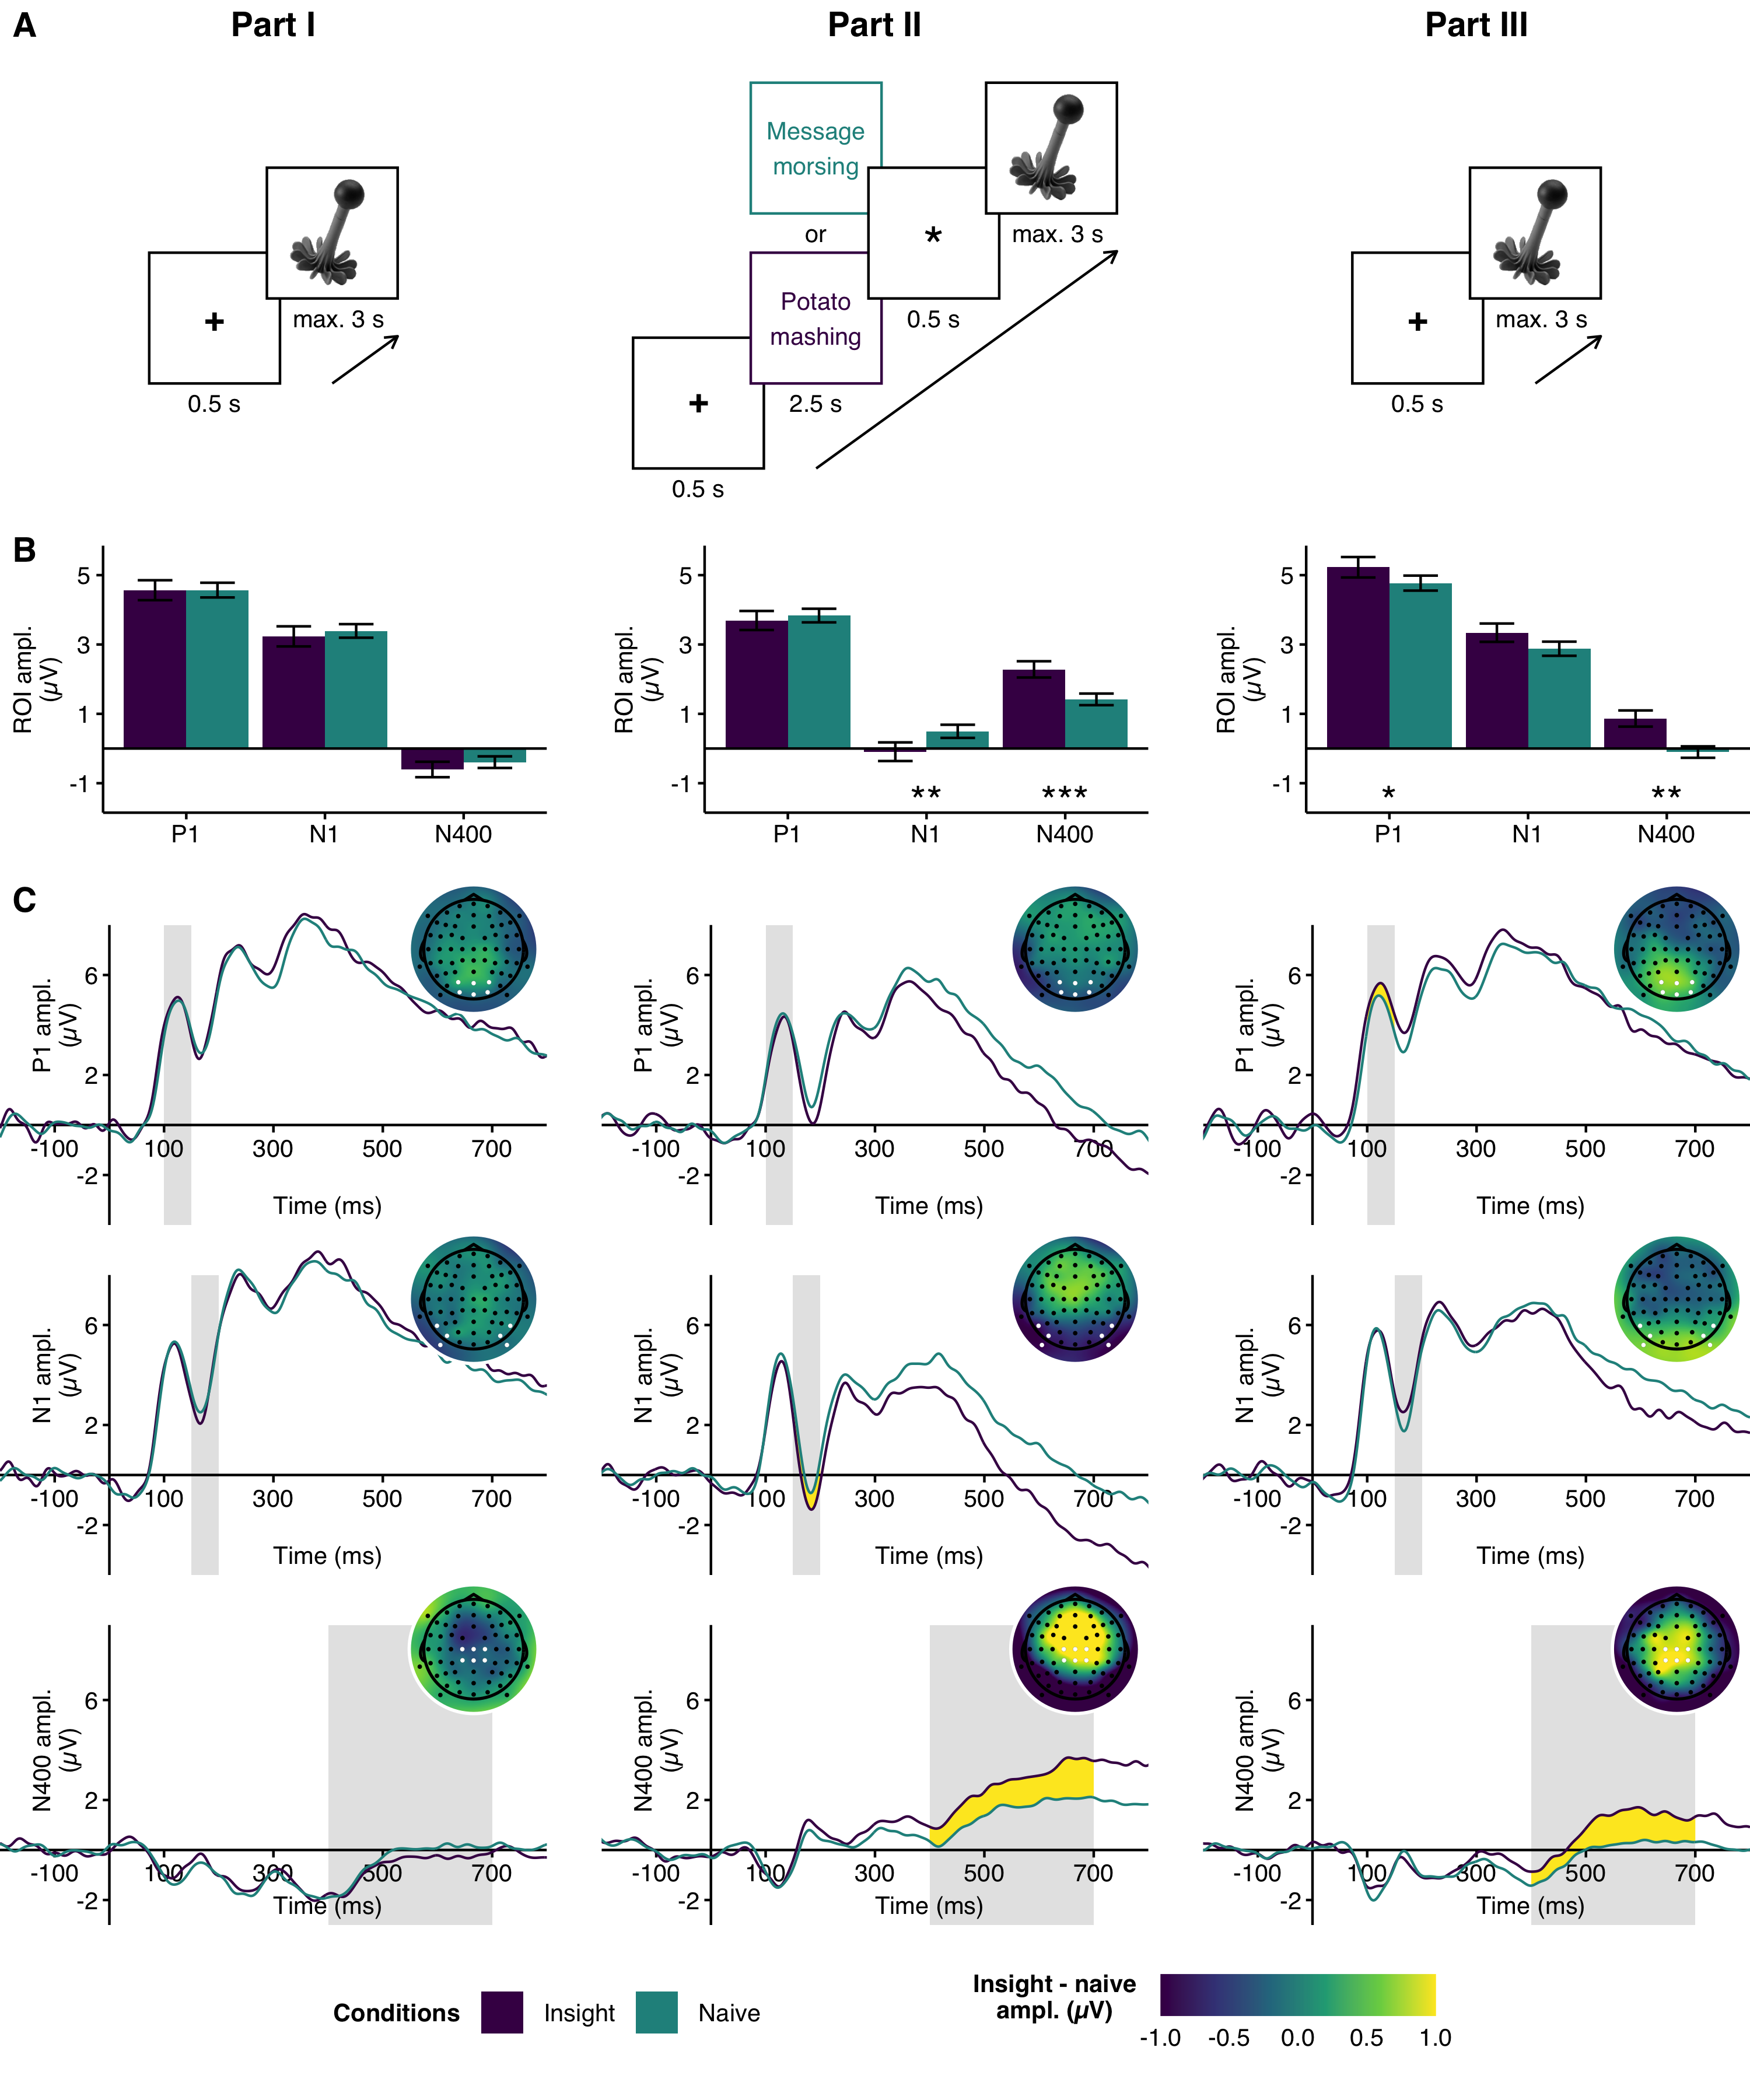
\includegraphics{manuscript_files/figure-latex/exp1-plot-1} 

}

\caption{Procedure and results of Experiment 1. (A) In Part I, participants viewed 120 unfamiliar objects and indicated whether they the object they were viewing. In Part II, half of the objects were preceded by a matching description (purple color, for illustrative purposes only), leading to semantic insight, and the other half with a non-matching description (petrol color, for illustrative purposes only), leading to naive perception. In Part III, the same objects were presented again without the descriptions. (B) Bar plots and (C) ERP waveforms and scalp topographies separately for objects for which participants experienced semantic insight and naive perception in Parts I, II, and III. Semantic insight was associated with significantly more negative amplitudes in the N1 component in Part II, significantly less negative amplitudes in the N400 component in Parts II and III, and significantly more positive amplitudes in the P1 component in Part III. Error bars show standard errors of the mean. \newline*\emph{p} \textless{} .05. **\emph{p} \textless{} .01. ***\emph{p} \textless{} .001.}\label{fig:exp1-plot}
\end{figure}

In Part II, only the 120 unfamiliar objects were presented for a second time, now preceded either by a matching verbal description (in the insight condition) or by a non-matching verbal description (in the naive condition). Each trial consisted of a fixation cross presented for 0.5 s, followed by the presentation of the verbal description for 2.5 s. Then, an asterisk was presented in the middle of the screen for another 0.5 s, followed by the presentation of the object until a response was made or until a time out after 3 s. The objects were presented in blocks of 30 trials so that (a) there were 15 objects from each of the two experimental conditions and (b) objects within each block were heterogeneous in terms of their shape, visual complexity, and functional category (e.g.~medical devices, musical instruments). To make sure that insight indeed did (did not) occur in the insight (naive) condition, we excluded any objects from the insight condition if participants indicated not knowing the object or having rather no assumption (despite reading the matching description) and any objects from the naive condition if participants indicated knowing the object or having an assumption (despite reading the non-matching description). This resulted in an average of 27.0 objects (44.9\%) per participant in the insight condition and an average of 48.8 objects (81.2\%) per participant in the naive condition.

In Part III, the unfamiliar objects were presented for a third time with an identical trial structure as in Part I, i.e.~without the verbal descriptions. Note that Parts II and III were presented in an interleaved fashion so that after the presentation of one block of 30 objects in Part II (with descriptions), participants took a self-timed break and continued with the same block of 30 objects in Part III (without descriptions) before moving on to the next block consisting of 30 different objects. They continued like this until all four blocks were completed in both Parts II and III. In total, the experiment consisted of 480 trials (120 familiar objects in Part I and 120 unfamiliar objects in Parts I, II, and III) and took participants approximately 35 minutes to complete.

\hypertarget{eeg-recording-and-preprocessing}{%
\subsubsection{EEG Recording and Preprocessing}\label{eeg-recording-and-preprocessing}}

The continuous EEG was recorded from 62 Ag/AgCl scalp electrodes placed according to the extended 10--20 system (American Electroencephalographic Society, 1991) and referenced online to an external electrode placed on the left mastoid (M1). Two additional external electrodes were placed on the right mastoid (M2) and below the left eye (IO1), respectively. During the recording, electrode impedances were kept below 5 kΩ. An online bandpass filter with a high-pass time-constant of 10 s (0.016 Hz) and a low-pass cutoff frequency of 1,000 Hz was applied before digitizing the signal at a sampling rate of 500 Hz.

Offline, the data were preprocessed using the MNE software (Version 0.20.8; Gramfort et al., 2013) in Python (Version 3.7.7; van Rossum \& Drake, 2009). First, all scalp electrodes were re-referenced to the common average. Next, artifacts from blinks and eye movements were removed using independent component analysis (ICA). The first 15 components were extracted using the FastICA algorithm (Hyvärinen, 1999) after temporarily low-pass filtering the data at 1 Hz. Those components showing substansive correlations with either of two virtual EOG channels (VEOG: IO1 minus Fp1, HEOG: F9 minus F10) were removed automatically using the \emph{find\_bads\_eog} function. After artifact correction, a zero-phase, non-causal FIR filter with a lower passband edge at 0.1 Hz (transition bandwidth: 0.1 Hz) and an upper passband edge at 30 Hz (transition bandwidth: 7.5 Hz) was applied. Next, the continuous EEG was epoched into segments of 2,000 ms, starting 500 ms before the onset of the visual presentation of each unfamiliar object. The epochs were baseline-corrected by substracting the average activity during the 200 ms before stimulus onset. Epochs containing artifacts despite ICA (defined as peak-to-peak amplitudes exceeding 200 µV) were removed from further analysis. This led to the exclusion of an average of 2.4 trials (0.7\%) per participant (range 0 to 24). Single-trial event-related potentials were computed as the mean amplitude across time windows and regions of interests (ROIs) defined a priori, namely 100--150 ms after object onset at electrodes PO3, PO4, POz, O1, O2, and Oz for the P1 component, 150--200 ms after object onset at electrodes P7, P8, PO7, PO8, PO9, and PO10 for the N1 component, and 400--700 ms at electrodes C1, C2, Cz, CP1, CP2, and CPz for the N400 component.

\hypertarget{statistical-analysis}{%
\subsubsection{Statistical Analysis}\label{statistical-analysis}}

The event-related potentials were analyzed on the single trial level using linear mixed-effects regression models (Baayen et al., 2008; Frömer et al., 2018). For the purpose of the present study, these models have a number of desirable properties compared to more traditional approaches, such as analyses of variance (ANOVAs) performed on by-participant grand averages. First, they can account simultanously for the non-independence of data points coming from the same participant or from the same item, whereas the neglect of item as a random variable in ANOVAs leads to anti-conservative test statistics and strictly does not allow for inferences beyond the stimulus set under study (Bürki et al., 2018; Judd et al., 2012). Second, they can flexibly deal with unbalanced designs in which the number of trials differs across (combinations of) conditions, which is inevitable in designs where the assignment of trials to conditions is based on the participants' responses rather than on the experimental manipulation (e.g.~Fröber et al., 2017).

Three separate models were computed predicting P1, N1, and N400 mean amplitudes. All models included three fixed effects: (a) the part of the experiment, coded as a sliding difference contrast (i.e.~subtracting Part I from Part II and Part II from Part III, the intercept being the grand mean across all three parts), (b) the condition of the trial, coded as a simple contrast (i.e.~subtracting the naive from the insight condition, the intercept being the grand mean across both conditions), and (c) the two-way interaction of part and condition. To determine the random effects structure, we always started with a model containing by-participant and by-item random intercepts and random slopes for all fixed effects (Barr et al., 2013). To increase statistical power and to avoid overfitting, we then iteratively removed each random effects term and re-added it only if the resulting model fitted the data significanlty worse than the maximal model as indicated by likelihood ratio tests (Matuschek et al., 2017). All models were fitted in R (Version 4.0.2; R Core Team, 2020) using the lme4 package (Version 1.1.23; Bates et al., 2015). The optimizer function \emph{bobyqa} with 2·10\textsuperscript{6} iterations was used for maximum likelihood estimation. Model selection via likelihood ratio tests was performed using the buildmer package (Version 1.7.1; Voeten, 2020). Finally, to answer the research question of whether or not semantic insight had an influence on the ERP components within each part, planned follow-up comparisons contrasting the insight versus the naive condition within Parts I, II, and III were calculated.

All materials and code for the present experiments can be accessed via the Open Science Framework (\href{https://osf.io/myprojects/}{https://osf.io/\ldots/}).

\hypertarget{results}{%
\subsection{Results}\label{results}}

Single-trial ERPs were analyzed in response to unfamiliar objects before (Part I), during (Part II), and after (Part III) participants gained semantic insight into what the objects were doing. Half the objects were preceded by a matching description, fostering semantic insight to occur, whereas the other half were preceded by non-matching description, leading to naive perception of the object. To make sure participants did indeed experience insight or naive perception, the analysis was constrained by participants' behavioral responses in Part II: Objects presented with matching a description were assigned to the insight condition only if the participant indicated that they knew what the object was doing (or had an assumption), whereas objects presented with a non-matching description were assigned to the naive condition only if the participant indicated that they did not know what the object was (or had rather no assumption). The analysis focused on differences between the insight and the naive condition in the P1 component (100--150 ms) as an index of low-level visual perception, in the N1 component (150--200 ms) as index of high-level visual perception, and in the N400 component (400--700 ms) as an index of semantic processing.

\begin{table}[tbp]

\begin{center}
\begin{threeparttable}

\caption{\label{tab:exp1-table}Results of linear mixed-effects regression models for Experiment 1}

\footnotesize{

\begin{tabular}{lcccccc}
\toprule
 & \multicolumn{2}{c}{\textbf{P1}} & \multicolumn{2}{c}{\textbf{N1}} & \multicolumn{2}{c}{\textbf{N400}} \\
\cmidrule(r){2-3} \cmidrule(r){4-5} \cmidrule(r){6-7}
\textit{Fixed effects} & \textit{F} (\textit{df}) & \textit{p} & \textit{F} (\textit{df}) & \textit{p} & \textit{F} (\textit{df}) & \textit{p}\\
\midrule
Part & 10.82 (2, 24.5) & < .001 & 14.15 (2, 24.9) & < .001 & 33.00 (2, 25.5) & < .001\\
Insight & 0.87 (1, 5302.9) & .351 & 0.96 (1, 5344.3) & .327 & 21.82 (1, 5214.0) & < .001\\
Pt. × ins. & 2.40 (2, 4590.9) & .091 & 5.33 (2, 4940.9) & .005 & 11.16 (2, 5055.1) & < .001\\
\textit{Insight $-$  naive} & Est. [95\% CI] & \textit{p} & Est. [95\% CI] & \textit{p} & Est. [95\% CI] & \textit{p}\\ \midrule
Part I & 0.00 [-0.50, 0.49] & .987 & -0.16 [-0.62, 0.30] & .485 & -0.21 [-0.61, 0.18] & .292\\
Part II & -0.15 [-0.65, 0.34] & .550 & -0.66 [-1.12, -0.20] & .005 & 0.91 [0.51, 1.31] & < .001\\
Part III & 0.57 [0.08, 1.07] & .023 & 0.41 [-0.05, 0.87] & .080 & 0.99 [0.58, 1.39] & < .001\\
\bottomrule
\addlinespace
\end{tabular}

}

\begin{tablenotes}[para]
\normalsize{\textit{Note.} Pt. = part, ins. = insight, est. = estimate, CI = confidence interval.}
\end{tablenotes}

\end{threeparttable}
\end{center}

\end{table}

Averaged accross conditions, P1, N1, and N400 amplitudes differed as a function of the part of the experiment, all \emph{F}s \textgreater{} 10.82, all \emph{p}s \textless{} .001 (Table \ref{tab:exp1-table}). In addition, N400 amplitudes differed between the insight and the naive conditions averaged across the three parts of the experiment, \emph{F}(1, 5214.0) = 21.82. Crucially, the part × insight interaction was significant in the N1, \emph{F}(2, 4940.9) = 5.33, \emph{p} = .005, and in the N400, \emph{F}(2, 5055.1) = 11.16, \emph{p} \textless{} .001, while also being marginally significant in the P1, \emph{F}(2, 4590.9) = 2.40, \emph{p} = .091. To answer our main research question, we decomposed these interactions into the differences between the insight and the naive condition within the three different parts of the experiment.

\hypertarget{effects-of-insight-in-part-i}{%
\subsubsection{Effects of Insight in Part I}\label{effects-of-insight-in-part-i}}

In Part I, when all objects were unfamiliar to the participants and presented without verbal descriptions, no differences emerged between the insight and the naive condition in the P1, N1, or N400 component, all \emph{p}s \textgreater{} .292 (Table \ref{tab:exp1-table}, Figure \ref{fig:exp1-plot}B--D). On the one hand, this was to be expected given that the critical presentation of the descriptions (leading to semantic insight vs.~naive perception) had not yet taken place. On the other hand, the absence of reliable differences in Part I can be taken as evidence---with the usual caveats when interpreting null effects---that any subsequent effects of insight in Parts II and III cannot be explained solely by visual differences between the objects in the two conditions. Although the presentation of a matching or non-matching description for each object was counterbalanced across participants, the fact that different numbers of objects were excluded from the two conditions based on participants self report in Part II would have made it possible for such visual differences to emerge as a confounding factor. If they did, however, one would expect to detect them even before any descriptions were presented, which we now know was not the case.

\hypertarget{effects-of-insight-in-part-ii}{%
\subsubsection{Effects of Insight in Part II}\label{effects-of-insight-in-part-ii}}

In Part II, half of the unfamiliar objects were presented with matching verbal description (in the insight condition) and the other half were presented with non-matching verbal descriptions (in the naive condition). In response to objects for which participants experienced insight, the amplitude of the N1 component was significantly enlarged (i.e.~more negative), \emph{b} = -0.66, \emph{p} = .005, and the amplitude of the N400 component was significantly reduced (i.e.~less negative), \emph{b} = 0.91, \emph{p} \textless{} .001, compared to objects which participants viewed naively. As in Part I, there were no reliable differences in the P1 component, \emph{p} = .550.

\hypertarget{effects-of-insight-in-part-iii}{%
\subsubsection{Effects of Insight in Part III}\label{effects-of-insight-in-part-iii}}

In Part III, the unfamiliar objects were presented for a third time, again without the verbal descriptions (as in Part I) to test whether the occurence of semantic insight had any lasting effects on the perception of the objects. As in Part II, the N400 component remained significantly reduced in response to objects for which semantic insight had occurred, \emph{b} = 0.99, \emph{p} \textless{} .001, whereas the effect of insight in the N1 component did not reocurr, \emph{p} = .080. Instead, we now observed an even earlier modulation in the P1 component, which was significantly enlarged (i.e.~more positive) in response to objects for which semantic insight had occured, \emph{b} = 0.57, \emph{p} = .023.

\hypertarget{discussion}{%
\subsection{Discussion}\label{discussion}}

In Experiment 1, we measured event-related brain potentials from participants viewing unfamiliar objects before (Part I), while (Part II) and after (Part III) they gained semantic insight into what kind of object they were seeing. To induce insight, half of the objects in Part II were preceded by a matching verbal description of the object's typical function or use, whereas the other half were preceded by a non-matching description (as a naive baseline condition).

Participants' experience of semantic insight in Part II was associated with a significantly larger N1 component, indicating that the sudden acquisition of knowledge about the object influenced aspects of its high-level visual processing (Rossion \& Jacques, 2011; Tanaka \& Curran, 2001). The fact that this effect did not reocurr in Part III, when the objects were presented once more without descriptions, suggests its role as a marker of semantic insight altering object processing online. In contrast, we also observed a modulation of the N400 component, which was reduced for objects when semantic insight was ocurring (in Part II) and remained so when the same objects were presented repeatedly (in Part III). The N400 is often viewed as an index of increased demands for semantic processing (Kutas \& Federmeier, 2011; Rabovsky et al., 2018). Its reduction can thus be interpreted as lower semantic processing demands in response to unfamiliar objects once participants had unterstood what kind of objects they were viewing. Finally, semantic insight was also associated with increased amplitudes in the P1 component, but once the objects were repeated again (in Part III) after the critical presentation during which semantic insight had ocurred (in Part II). This effect, which replicates previous work on obtaining knowledge about previously unfamiliar images (Samaha et al., 2018), may be associated with the newly acquired semantic knowledge exerting an influence on lower-level visual perception, either online or through altered visual representations of the objects for which insight had ocurred.

However, because of the exploratory nature of the present study and the novelty of the ERP effects observed in Experiment 1, we first ran a replication study to assess the robustness of these findings in another samples of participants.

\hypertarget{experiment-2}{%
\section{Experiment 2}\label{experiment-2}}

\hypertarget{methods-1}{%
\subsection{Methods}\label{methods-1}}

\hypertarget{participants-1}{%
\subsubsection{Participants}\label{participants-1}}

Participants for Experiment 2 were 24 German native speakers (18 female, 6 male) with a mean age of 23 years (range 19 to 32) who had not participated in Experiment 1. They had no history of psychological disorder or treatment, were right-handed and reported normal or corrected-to-normal vision. They gave written informed consent before starting the experiment and received a compensation of €8 per hour for participating.

\hypertarget{materials-procedure-and-analysis}{%
\subsubsection{Materials, Procedure, and Analysis}\label{materials-procedure-and-analysis}}

All materials, procedures, and methods for EEG recording and statistical analysis were identical to Experiment 1. An average of 5.8\% of rare objects per participant was classified as known in Part I and excluded from all further analyses. Based on participants' responses in Part II, an average of 26.4 objects (44.9\% of objects presented with matching descirptions) were assigned to the insight condition and an average of 49.2 objects (81.2\% of objects presented with non-matching descriptions) were assigned to the naive condition. Automatic rejection of EEG epochs containing artifacts led to the exlucsion of 11.0 trials (3.0\%) per participant (range 0 to 85).

\hypertarget{results-1}{%
\subsection{Results}\label{results-1}}

\begin{table}[tbp]

\begin{center}
\begin{threeparttable}

\caption{\label{tab:exp2-table}Results of linear mixed-effects regression models for Experiment 2}

\footnotesize{

\begin{tabular}{lcccccc}
\toprule
 & \multicolumn{2}{c}{\textbf{P1}} & \multicolumn{2}{c}{\textbf{N1}} & \multicolumn{2}{c}{\textbf{N400}} \\
\cmidrule(r){2-3} \cmidrule(r){4-5} \cmidrule(r){6-7}
\textit{Fixed effects} & \textit{F} (\textit{df}) & \textit{p} & \textit{F} (\textit{df}) & \textit{p} & \textit{F} (\textit{df}) & \textit{p}\\
\midrule
Part & 18.14 (2, 5151.1) & < .001 & 16.39 (2, 25.0) & < .001 & 70.58 (2, 25.2) & < .001\\
Insight & 0.03 (1, 5272.5) & .853 & 1.23 (1, 5218.6) & .267 & 18.66 (1, 5207.5) & < .001\\
Pt. × ins. & 3.74 (2, 5151.2) & .024 & 1.34 (2, 4736.8) & .263 & 8.07 (2, 4637.6) & < .001\\
\textit{Insight $-$  naive} & Est. [95\% CI] & \textit{p} & Est. [95\% CI] & \textit{p} & Est. [95\% CI] & \textit{p}\\ \midrule
Part I & -0.17 [-0.72, 0.38] & .552 & -0.04 [-0.53, 0.45] & .864 & 0.02 [-0.44, 0.48] & .936\\
Part II & -0.49 [-1.04, 0.07] & .084 & -0.50 [-0.99, 0.00] & .050 & 1.31 [0.86, 1.77] & < .001\\
Part III & 0.56 [0.01, 1.11] & .048 & 0.04 [-0.45, 0.54] & .865 & 0.45 [-0.01, 0.91] & .055\\
\bottomrule
\addlinespace
\end{tabular}

}

\begin{tablenotes}[para]
\normalsize{\textit{Note.} Pt. = part, ins. = insight, est. = estimate, CI = confidence interval.}
\end{tablenotes}

\end{threeparttable}
\end{center}

\end{table}

As in Experiment 1, P1, N1, and N400 amplitudes differed between the three different parts of the experiments, all \emph{F}s \textgreater{} 16.39, all \emph{p}s \textless{} .001 (Table \ref{tab:exp2-table}). Also as in Experiment 1, N400 amplitudes differed between the insight and the naive condition averaged across parts, \emph{F}(1, 5207.5) = 18.66. The part × insight interaction was significant in the P1, \emph{F}(2, 5151.2) = 3.74, \emph{p} = .024, and in the N400, \emph{F}(2, 4637.6) = 8.07, \emph{p} \textless{} .001, but not in the N1, \emph{F}(2, 4736.8) = 1.34, \emph{p} = .263.

\begin{figure}

{\centering 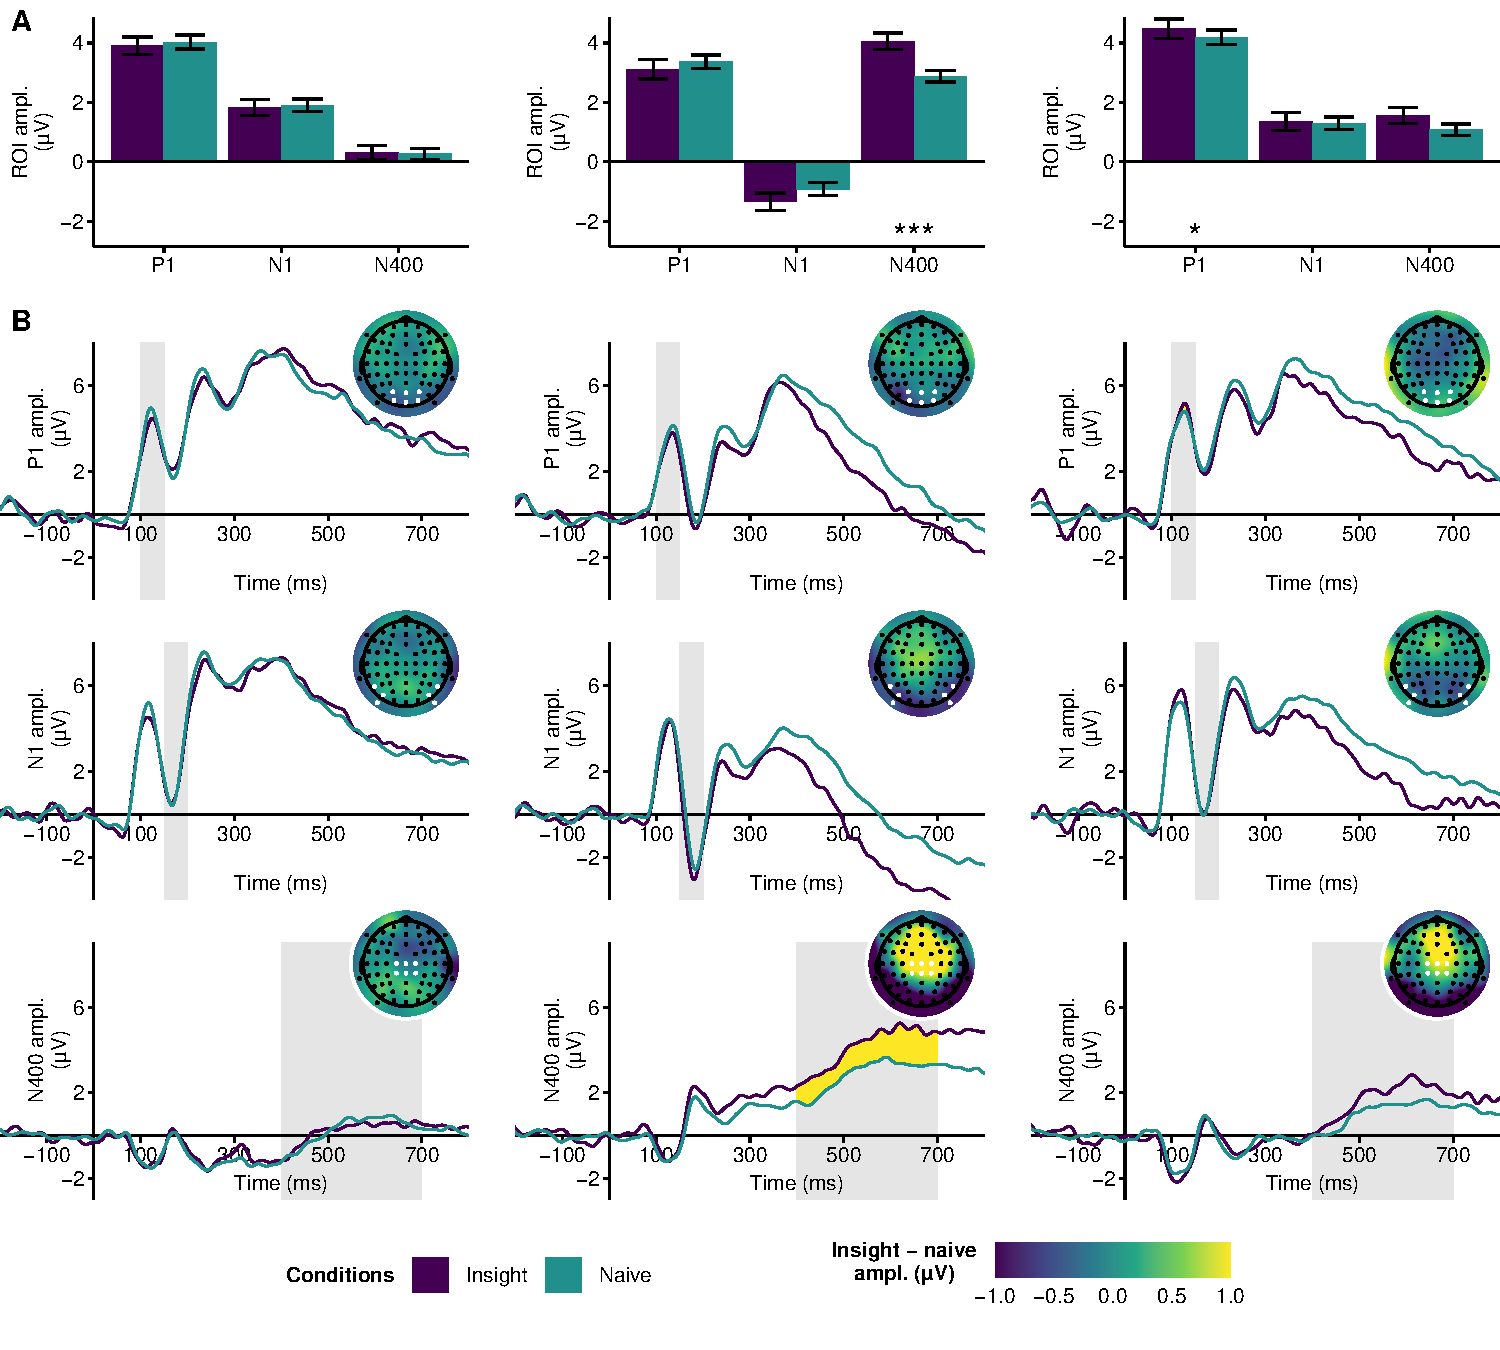
\includegraphics{manuscript_files/figure-latex/exp2-plot-1} 

}

\caption{Results of Experiment 2. A. Bar plots and B. ERP waveforms and scalp topographies separately for objects for which participants experienced semantic insight and naive perception in Parts I, II, and III. In a direct replication of Experiment 1, the effect of semantic insight on the N400 component in Part II and on the P1 component in Part III remained statistically significant, while the effect on the N1 component in Part II and on the N400 component in Part III remained only marginally significant. \newline*\emph{p} \textless{} .05. ***\emph{p} \textless{} .001.}\label{fig:exp2-plot}
\end{figure}

\hypertarget{effects-of-insight-in-part-i-1}{%
\subsubsection{Effects of Insight in Part I}\label{effects-of-insight-in-part-i-1}}

As in Experiment 1, no differences between objects in the insight and the naive condition emerged in the P1, N1, or N400 component, all \emph{p}s \textgreater{} .552 (Table \ref{tab:exp2-table}, Figure \ref{fig:exp2-plot}).



\hypertarget{effects-of-insight-in-part-ii-1}{%
\subsubsection{Effects of Insight in Part II}\label{effects-of-insight-in-part-ii-1}}

As in Experiment 1, the occurence of semantic insight in Part II due to the presentation of objects with matching (vs.~non-matching) verbal descriptions was associated with a (marginally) significant enhancement of the N1 component, \emph{b} = -0.50, \emph{p} = .050, and a signficant reduction of the N400 component, \emph{b} = 0.91, \emph{p} \textless{} .001.

\hypertarget{effects-of-insight-in-part-iii-1}{%
\subsubsection{Effects of Insight in Part III}\label{effects-of-insight-in-part-iii-1}}

As in Experiment 1, the presentation of the same unfamiliar objects for a third time (without verbal descriptions as in Part I) led to significantly larger amplitudes in the P1 component in response to objects for which semantic insight had occured, \emph{b} = 0.56, \emph{p} = .048. Also, the N400 amplitude in response to these objects remained reduced, although marginally significant, \emph{b} = 0.45, \emph{p} .055.

\hypertarget{joint-analysis-of-experiments-1-and-2}{%
\subsubsection{Joint Analysis of Experiments 1 and 2}\label{joint-analysis-of-experiments-1-and-2}}

In an attempt to maximize statistical power, we combined the data sets from Experiments 1 and 2. This allowed us to determine (a) if the above effects---including the marginally significant ones---were reliable when tested in a larger sample, and (b) if there were significant differences in the ERP amplitudes between Experiments 1 and 2. Methods for statistical analysis were kept the same as above, despite the addition of a new factor for experiment, coded as a simple contrast (i.e.~subtracting the Experiment 1 from Experiment 2, the intercept being the grand mean across both experiments). This factor and its possible interactions with part, insight, and part × insight were included in the linear mixed-effects regression models as fixed effects and as potential by-item random effects. Note that, as above, random effects were included only if their omission led to a significant decline in model fit (Matuschek et al., 2017).

\begin{table}[tbp]

\begin{center}
\begin{threeparttable}

\caption{\label{tab:joint-table}Results of linear mixed-effects regression models for Experiments 1 and 2 combined}

\footnotesize{

\begin{tabular}{lcccccc}
\toprule
 & \multicolumn{2}{c}{\textbf{P1}} & \multicolumn{2}{c}{\textbf{N1}} & \multicolumn{2}{c}{\textbf{N400}} \\
\cmidrule(r){2-3} \cmidrule(r){4-5} \cmidrule(r){6-7}
\textit{Fixed effects} & \textit{F} (\textit{df}) & \textit{p} & \textit{F} (\textit{df}) & \textit{p} & \textit{F} (\textit{df}) & \textit{p}\\
\midrule
Part & 12.38 (2, 49.0) & < .001 & 29.89 (2, 50.0) & < .001 & 95.34 (2, 50.6) & < .001\\
Insight & 0.35 (1, 10560.3) & .552 & 1.77 (1, 10560.5) & .183 & 38.72 (1, 10518.8) & < .001\\
Experiment & 0.35 (1, 48.2) & .555 & 2.39 (1, 48.1) & .129 & 4.75 (1, 48.4) & .034\\
Pt. × ins. & 4.02 (2, 9042.4) & .018 & 5.59 (2, 9966.0) & .004 & 15.73 (2, 10010.1) & < .001\\
Pt. × exp. & 0.03 (2, 49.0) & .971 & 0.55 (2, 50.0) & .581 & 2.58 (2, 50.6) & .086\\
Ins. × exp. & 0.62 (1, 10536.2) & .432 & 0.04 (1, 10501.0) & .836 & 0.03 (1, 10574.9) & .865\\
Pt. × ins. × exp. & 0.03 (2, 9042.9) & .972 & 0.62 (2, 9966.2) & .536 & 2.65 (2, 10010.4) & .070\\
\textit{Insight $-$  naive} & Est. [95\% CI] & \textit{p} & Est. [95\% CI] & \textit{p} & Est. [95\% CI] & \textit{p}\\ \midrule
Part I & -0.07 [-0.44, 0.30] & .699 & -0.10 [-0.43, 0.24] & .565 & -0.10 [-0.41, 0.20] & .507\\
Part II & -0.22 [-0.59, 0.15] & .248 & -0.56 [-0.90, -0.22] & .001 & 1.09 [0.79, 1.39] & < .001\\
Part III & 0.49 [0.12, 0.86] & .010 & 0.25 [-0.09, 0.59] & .148 & 0.72 [0.41, 1.02] & < .001\\
\bottomrule
\addlinespace
\end{tabular}

}

\begin{tablenotes}[para]
\normalsize{\textit{Note.} Pt. = part, ins. = insight, exp. = experiment, est. = estimate, CI = confidence interval.}
\end{tablenotes}

\end{threeparttable}
\end{center}

\end{table}

As shown in Table \ref{tab:joint-table}, all main effects for part in the P1, N1, and N400 were significant, all \emph{F}s \textgreater{} 12.38, all \emph{p}s \textless{} .001, as was the main effect of insight in the N400, \emph{F}(1, 10518.8) = 38.72, \emph{p} \textless{} .001. Furthermore, the part × insight now was reliably observed in all three components, all \emph{F}s \textgreater{} 4.02, all \emph{p}s \textless{} .018. While there was a main effect of experiment in the N400, \emph{F}(1, 48.4) = 4.75, \emph{p} = .034, the absence of any reliable interactions of experiment with part or insight indicated that the effect of our experimental manipulations did not differ between Experiments 1 and 2.

We therefore computed the same planned comparisons between the insight and the naive condition within each part, now collapsed across the data from both experiments. This confirmed the absence of any reliable difference between the two conditions in Part I, all \emph{p}s \textgreater{} .507, the significant enhancement in the N1 in Part II, while insight was ocurring, \emph{b} = -0.56, \emph{p} = .001, the significant reduction in the N400 for insight in Parts II, while insight was occurring, \emph{b} = 1.09, \emph{p} \textless{} .001, and Part III, after insight had ocurred, \emph{b} 0.72, \emph{p} = \textless{} .001, as well as the sigificant enhancement in the P1 in Part III, after insight had occurred, \emph{b} = 0.49, \emph{p} = .010.

\hypertarget{discussion-1}{%
\subsection{Discussion}\label{discussion-1}}

Experiment 2, a direct replication of Experiment 1, confirmed the impact of gaining the semantic insight into previously unfamiliar objects on ERPs associated with low-level visual perception (P1), high-level visual perception (N1), and semantic processing (N400). While the enhancement of the N1, being more negative in repsonse to objects for which participants experienced semantic insight, was present only during the critical presentation of the objects with their verbal descriptions (in Part II), the enhancement of the P1, being more positive in response to these same objects, emerged only after insight had taken place and the objects were presented again in Part III. This indicates a modulation of different stages of visual perception of objects through semantic knowledge while and after an understanding of the object has been obtained. Finally, a sustained reduction of the N400 component in response to objects for which participants experienced semantic insight may reflect lesser semantic processing demands as compared to unfamiliar objects which participants did not yet understand.

\hypertarget{experiment-3}{%
\section{Experiment 3}\label{experiment-3}}

\newpage

\hypertarget{references}{%
\section{References}\label{references}}

\begingroup
\setlength{\parindent}{-0.5in}
\setlength{\leftskip}{0.5in}

\hypertarget{refs}{}
\begin{cslreferences}
\leavevmode\hypertarget{ref-americanelectroencephalographicsociety1991}{}%
American Electroencephalographic Society. (1991). American Electroencephalographic Society guidelines for standard electrode position nomenclature. \emph{Journal of Clinical Neurophysiology}, \emph{8}(2), 200--202.

\leavevmode\hypertarget{ref-baayen2008}{}%
Baayen, R. H., Davidson, D. J., \& Bates, D. M. (2008). Mixed-effects modeling with crossed random effects for subjects and items. \emph{Journal of Memory and Language}, \emph{59}(4), 390--412. \url{https://doi.org/10.1016/j.jml.2007.12.005}

\leavevmode\hypertarget{ref-barr2013}{}%
Barr, D. J., Levy, R., Scheepers, C., \& Tily, H. J. (2013). Random effects structure for confirmatory hypothesis testing: Keep it maximal. \emph{Journal of Memory and Language}, \emph{68}(3), 255--278. \url{https://doi.org/10.1016/j.jml.2012.11.001}

\leavevmode\hypertarget{ref-R-lme4}{}%
Bates, D., Mächler, M., Bolker, B., \& Walker, S. (2015). Fitting linear mixed-effects models using lme4. \emph{Journal of Statistical Software}, \emph{67}(1), 1--48. \url{https://doi.org/10.18637/jss.v067.i01}

\leavevmode\hypertarget{ref-buxfcrki2018}{}%
Bürki, A., Frossard, J., \& Renaud, O. (2018). Accounting for stimulus and participant effects in event-related potential analyses to increase the replicability of studies. \emph{Journal of Neuroscience Methods}, \emph{309}, 218--227. \url{https://doi.org/10.1016/j.jneumeth.2018.09.016}

\leavevmode\hypertarget{ref-fruxf6ber2017}{}%
Fröber, K., Stürmer, B., Frömer, R., \& Dreisbach, G. (2017). The role of affective evaluation in conflict adaptation: An LRP study. \emph{Brain and Cognition}, \emph{116}, 9--16. \url{https://doi.org/10.1016/j.bandc.2017.05.003}

\leavevmode\hypertarget{ref-fruxf6mer2018}{}%
Frömer, R., Maier, M., \& Abdel Rahman, R. (2018). Group-level EEG-processing pipeline for flexible single trial-based analyses including linear mixed models. \emph{Frontiers in Neuroscience}, \emph{12}. \url{https://doi.org/10.3389/fnins.2018.00048}

\leavevmode\hypertarget{ref-gramfort2013}{}%
Gramfort, A., Luessi, M., Larson, E., Engemann, D. A., Strohmeier, D., Brodbeck, C., Goj, R., Jas, M., Brooks, T., Parkkonen, L., \& al. (2013). MEG and EEG data analysis with MNE-Python. \emph{Frontiers in Neuroscience}, \emph{7}. \url{https://doi.org/10.3389/fnins.2013.00267}

\leavevmode\hypertarget{ref-hyvuxe4rinen1999}{}%
Hyvärinen, A. (1999). Fast and robust fixed-point algorithms for independent component analysis. \emph{IEEE Transactions on Neural Networks}, \emph{10}(3), 626--634. \url{https://doi.org/10.1109/72.761722}

\leavevmode\hypertarget{ref-judd2012}{}%
Judd, C. M., Westfall, J., \& Kenny, D. A. (2012). Treating stimuli as a random factor in social psychology: A new and comprehensive solution to a pervasive but largely ignored problem. \emph{Journal of Personality and Social Psychology}, \emph{103}(1), 54--69. \url{https://doi.org/10.1037/a0028347}

\leavevmode\hypertarget{ref-kutas2011}{}%
Kutas, M., \& Federmeier, K. D. (2011). Thirty years and counting: Finding meaning in the n400 component of the event-related brain potential (erp). \emph{Annual Review of Psychology}, \emph{62}, 621--647. \url{https://doi.org/10.1146/annurev.psych.093008.131123}

\leavevmode\hypertarget{ref-matuschek2017}{}%
Matuschek, H., Kliegl, R., Vasishth, S., Baayen, H., \& Bates, D. (2017). Balancing Type I error and power in linear mixed models. \emph{Journal of Memory and Language}, \emph{94}, 305--315. \url{https://doi.org/10.1016/j.jml.2017.01.001}

\leavevmode\hypertarget{ref-oldfield1971}{}%
Oldfield, R. C. (1971). The assessment and analysis of handedness: The Edinburgh inventory. \emph{Neuropsychologia}, \emph{9}(1), 97--113. \url{https://doi.org/10.1016/0028-3932(71)90067-4}

\leavevmode\hypertarget{ref-rabovsky2018}{}%
Rabovsky, M., Hansen, S. S., \& McClelland, J. L. (2018). Modelling the n400 brain potential as change in a probabilistic representation of meaning. \emph{Nature Human Behaviour}, \emph{2}(9), 693--705. \url{https://doi.org/10.1038/s41562-018-0406-4}

\leavevmode\hypertarget{ref-R-base}{}%
R Core Team. (2020). \emph{R: A language and environment for statistical computing}. R Foundation for Statistical Computing. \url{https://www.R-project.org/}

\leavevmode\hypertarget{ref-rossion2011}{}%
Rossion, B., \& Jacques, C. (2011). The n170: Understanding the time course of face perception in the human brain. In \emph{The oxford handbook of event-related potential components} (pp. 115--142). Oxford University Press. \url{https://doi.org/10.1093/oxfordhb/9780195374148.001.0001}

\leavevmode\hypertarget{ref-samaha2018}{}%
Samaha, J., Boutonnet, B., Postle, B. R., \& Lupyan, G. (2018). Effects of meaningfulness on perception: Alpha-band oscillations carry perceptual expectations and influence early visual responses. \emph{Scientific Reports}, \emph{8}(1), 1--14. \url{https://doi.org/10.1038/s41598-018-25093-5}

\leavevmode\hypertarget{ref-tanaka2001}{}%
Tanaka, J. W., \& Curran, T. (2001). A neural basis for expert object recognition. \emph{Psychological Science}, \emph{12}(1), 43--47. \url{https://doi.org/10.1111/1467-9280.00308}

\leavevmode\hypertarget{ref-vanrossum2009}{}%
van Rossum, G., \& Drake, F. L. (2009). \emph{Python 3 reference manual}. CreateSpace.

\leavevmode\hypertarget{ref-R-buildmer}{}%
Voeten, C. C. (2020). \emph{buildmer: Stepwise elimination and term reordering for mixed-effects regression}. \url{https://CRAN.R-project.org/package=buildmer}
\end{cslreferences}

\endgroup


\end{document}
